% Beamer
  \documentclass{beamer}
  \usecolortheme{seagull}

% Tikz
  \usepackage{tikz}
  \usetikzlibrary{arrows}
  \usepackage{tikz-qtree}

% SVG
  \usepackage{svg}
  \setsvg{svgpath = images/}


% Meta
  \title{How do I Cryptography?}
  \subtitle{Personal Learning Goal Presentation}
  \author{Justus Perlwitz}

\AtBeginSection[]{
  \begin{frame}
    \begin{center}
      \insertsection
    \end{center}
  \end{frame}
}

\tikzstyle{message} = [
  draw,
  rectangle,
  minimum width=1.5cm,
  align=center,
]
\tikzstyle{empty} = [
  fill,
]
\tikzstyle{actor} = [
]

\begin{document}
  \begin{frame}
    {\titlepage}
  \end{frame}
  \begin{frame}
    \frametitle{Table of Contents}
    \tableofcontents[]
  \end{frame}
  \section{Attack Trees}
    \subsection{How to hack My Ecosia}
      \begin{frame}
        \frametitle{\insertsubsection}
        \makebox[\textwidth][c]{
          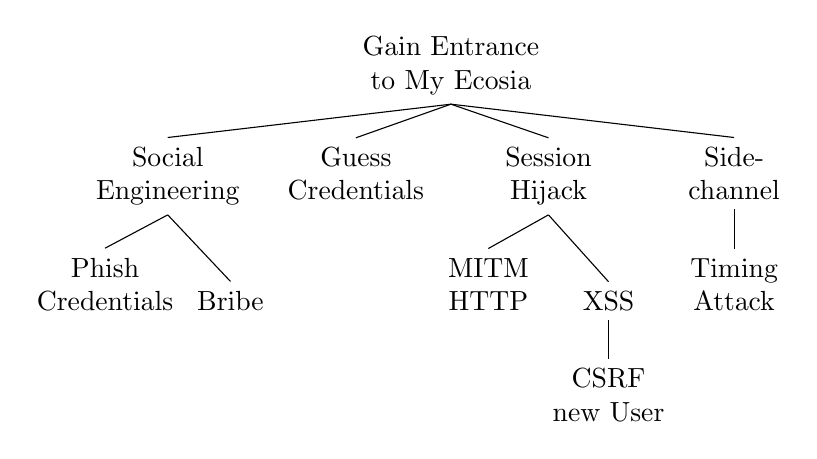
\begin{tikzpicture}[
            align=center,
            anchor=north,
            level distance=40pt,
          ]
          \Tree[
            .{Gain Entrance\\to My Ecosia}
            [
              .{Social\\Engineering}
              {Phish\\Credentials}
              Bribe
            ]
            {Guess\\Credentials}
            [
              .{Session\\Hijack}
              {MITM\\HTTP}
              [
                .{XSS}
                {CSRF\\new User}
              ]
            ]
            [
              .{Side-\\channel}
              {Timing\\Attack}
            ]
          ]
          \end{tikzpicture}
        }
      \end{frame}
      \begin{frame}
        \frametitle{Lessons learned}
        \begin{itemize}
          \item Do not use HTTP
          \item Block brute force attempts
          \item Educate employees about phishing
          \item CSRF cookies
          \item Use common cryptography patterns to avoid side-channel attacks
          \item Escape user submitted content (XSS, SQL Injections)
        \end{itemize}
      \end{frame}
      \subsection{Cryptography is not Security}
        \begin{frame}
          \frametitle{\insertsubsection}
          \begin{center}
            Implementing cryptography can go wrong very easily.
          \end{center}
        \end{frame}
  \section{Symmetric Encryption}
    \subsection{Problem}
      \begin{frame}
        \frametitle{\insertsubsection}
        Suppose \textit{Eve} wants to eavesdrop on \textit{Alice's} and \textit{Bob's}
        conversation.

        How can Alice send a message $m$ to Bob without Eve understanding $m$?

        \begin{center}
          \begin{tikzpicture}[
    auto,
  ]
  \matrix(m1)[
    ampersand replacement=\&,
    row sep=1cm,
    column sep=2cm,
  ]{
    \&
    \node[message]
    (evem){$m$};
    \&
    \\
    \node[message]
    (alicem){$m$};
    \&
    \node[empty](msg){};
    \&
    \node[message]
    (bobm){$m$};
    \\
  };
  \node[
    actor,
    above of=evem
  ](eve){Eve};
  \node[
    actor,
    above of=alicem,
  ](alice){Alice};
  \node[
    actor,
    above of=bobm
  ](bob){Bob};
  \path [] (alicem) edge node {} (msg);
  \path [->] (msg) edge node {$m$} (bobm);
  \path [->] (msg) edge node {$m$} (evem);
\end{tikzpicture}

        \end{center}
      \end{frame}
    \subsection{Definitions}
      \begin{frame}
        \frametitle{\insertsubsection}
        \begin{itemize}
          \item $K_e$: a secret key that Alice and Bob both agree on.
          \item $E(K_e ,m)$: the encryption function.
          \item $c$: the resulting ciphertext, with
          \item $c:=E(K_e ,m)$.
          \item $D(K_e ,c)$: the decrypting function, with
          \item $m = D(K_e, E(K_e , m))$.
        \end{itemize}
      \end{frame}
      \begin{frame}
        \frametitle{Generic Encryption}
        \begin{center}
          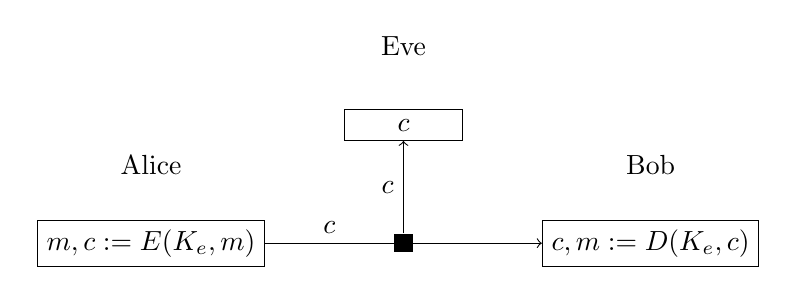
\begin{tikzpicture}[
    auto,
  ]
  \matrix(m1)[
    ampersand replacement=\&,
    row sep=1cm,
    column sep=1cm,
  ]{
    \&
    \node[message]
    (evem){$c$};
    \&
    \\
    \node[message]
    (alicem){$m, c:=E(K_e ,m)$};
    \&
    \node[empty](msg){};
    \&
    \node[message]
    (bobm){$c, m:= D(K_e ,c)$};
    \\
  };
  \node[
    actor,
    above of=evem
  ](eve){Eve};
  \node[
    actor,
    above of=alicem,
  ](alice){Alice};
  \node[
    actor,
    above of=bobm
  ](bob){Bob};
  \path [] (alicem) edge node {$c$} (msg);
  \path [->] (msg) edge node {} (bobm);
  \path [->] (msg) edge node {$c$} (evem);
\end{tikzpicture}

        \end{center}
      \end{frame}
      \begin{frame}
        \frametitle{Block Ciphers}
        \begin{enumerate}
          \item Block ciphers operate on blocks of plaintext with a fixed length.
          \item If necessary, blocks need to be padded to have the right length.
          \item There are various methods of applying block ciphers.
        \end{enumerate}
      \end{frame}
      \begin{frame}
        \frametitle{Electronic Code Book Mode}
        \resizebox{\textwidth}{!}{%
          \includesvg{ECB_encryption}%
        }
      \end{frame}
      \begin{frame}
        \frametitle{Cipher Block Chaining Mode}
        \resizebox{\textwidth}{!}{%
          \includesvg{CBC_encryption}%
        }
      \end{frame}
  \section{Authentication}
    \subsection{Problem}
      \begin{frame}
        \frametitle{\insertsubsection}
        How can Bob verify that a message $m$ really came from Alice?
        \begin{center}
          \begin{tikzpicture}[
    auto,
  ]
  \matrix(m1)[
    ampersand replacement=\&,
    row sep=1cm,
    column sep=2cm,
  ]{
    \&
    \node[message]
    (evem){$m^{\prime}$};
    \&
    \\
    \node[message]
    (alicem){$m$};
    \&
    \node[empty](msg){};
    \&
    \node[message]
    (bobm){$m^{\prime}$};
    \\
  };
  \node[
    actor,
    above of=evem
  ](eve){Eve};
  \node[
    actor,
    above of=alicem,
  ](alice){Alice};
  \node[
    actor,
    above of=bobm
  ](bob){Bob};
  \path [] (alicem) edge node {$m$} (msg);
  \path [->] (msg) edge node {$m^{\prime}$} (bobm);
  \path [->] (evem) edge node {} (msg);
\end{tikzpicture}

        \end{center}
      \end{frame}
    \subsection{Definitions}
      \begin{frame}
        \frametitle{\insertsubsection}
        Suppose Alice wants to send Bob the message $m$. We need to define
        the following:
        \begin{enumerate}
          \item $K_a$: secret authentication key shared between Alice and Bob.
          \item $a := h(K_a, m)$: the message authentication code (MAC)
        \end{enumerate}
      \end{frame}
      \begin{frame}
        \frametitle{Generic authentication}
        \begin{center}
          \begin{tikzpicture}[
    auto,
  ]
  \matrix(m1)[
    ampersand replacement=\&,
    row sep=1cm,
    column sep=1.5cm,
  ]{
    \&
    \node[message]
    (evem){$m^{\prime}$};
    \&
    \\
    \node[message]
    (alicem){$m,a:=h(K_a, m)$};
    \&
    \node[empty](msg){};
    \&
    \node[message]
    (bobm){$m,a \overset{?}{=}h(K_a, m)$};
    \\
  };
  \node[
    actor,
    above of=evem
  ](eve){Eve};
  \node[
    actor,
    above of=alicem,
  ](alice){Alice};
  \node[
    actor,
    above of=bobm
  ](bob){Bob};
  \path [] (alicem) edge node {$m$} (msg);
  \path [->] (msg) edge node {$m$} (bobm);
  \path [->] (evem) edge node {} (msg);
\end{tikzpicture}

        \end{center}
      \end{frame}
  \section{Asymmetric Encryption}
    \subsection{Problem}
      \begin{frame}
        \frametitle{\insertsubsection}
        How can Alice send a message to Bob without exchanging private keys?

        How can a group of people avoid having to exchange keys with each other?
      \end{frame}
    \subsection{Definitions}
      \begin{frame}
        \frametitle{\insertsubsection}
        Suppose Alice wants to send Bob the message $m$. We need to define
        the following:
        \begin{enumerate}
          \item $(S_{Bob}, P_{Bob})$: a keypair, with
          \item $S_{Bob}$ being the secret key that only Bob knows,
          \item $P_{Bob}$ being the public key that everyone knows.
          \item $D(S_{Bob}, E(P_{Bob}, m)) = m$ must hold.
        \end{enumerate}
      \end{frame}
      \begin{frame}
        \frametitle{Generic public-key encryption}
        \begin{center}
          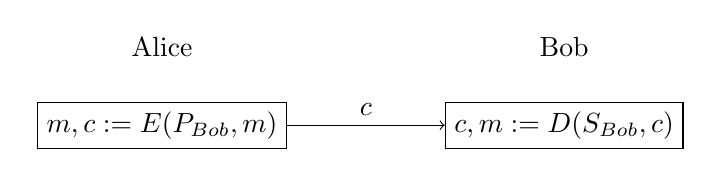
\begin{tikzpicture}[
    auto,
  ]
  \matrix(m1)[
    ampersand replacement=\&,
    row sep=1cm,
    column sep=2cm,
  ]{
    \node[message]
    (alicem){$m, c:=E(P_{Bob}, m)$};
    \&
    \node[message]
    (bobm){$c, m:= D(S_{Bob}, c)$};
    \\
  };
  \node[
    actor,
    above of=alicem,
  ](alice){Alice};
  \node[
    actor,
    above of=bobm
  ](bob){Bob};
  \path [->] (alicem) edge node {$c$} (bobm);
\end{tikzpicture}

        \end{center}
      \end{frame}
  \section{Digital Signatures}
    \subsection{Problem}
      \begin{frame}
        \frametitle{\insertsubsection}
        How can we send a message where the authenticity and integrity can be
        verified by everyone? How can we make sure that only one entity is able to
        send such messages?
      \end{frame}
    \subsection{Definitions}
      \begin{frame}
        \frametitle{\insertsubsection}
        Suppose Alice wants to send Bob a signed message. We need to define the
        following:
        \begin{enumerate}
          \item $(S_{Alice}, P_{Alice})$: Alice's keypair
          \item $s:=\sigma(S_{Alice}, m)$: The message signature
          \item $\upsilon(P_{Alice}, m, s)$: Verifies the signature.
        \end{enumerate}
      \end{frame}
      \begin{frame}
        \frametitle{Generic digital signature}
        \begin{center}
          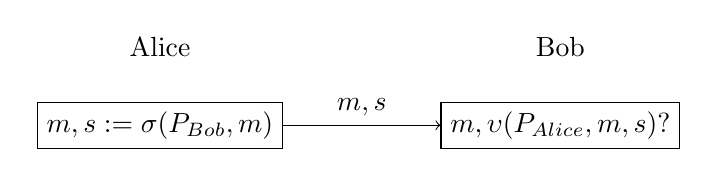
\begin{tikzpicture}[
    auto,
  ]
  \matrix(m1)[
    ampersand replacement=\&,
    row sep=1cm,
    column sep=2cm,
  ]{
    \node[message]
    (alicem){$m, s:=\sigma(P_{Bob}, m)$};
    \&
    \node[message]
    (bobm){$m, \upsilon(P_{Alice}, m, s)?$};
    \\
  };
  \node[
    actor,
    above of=alicem,
  ](alice){Alice};
  \node[
    actor,
    above of=bobm
  ](bob){Bob};
  \path [->] (alicem) edge node {$m, s$} (bobm);
\end{tikzpicture}

        \end{center}
      \end{frame}
\end{document}
